\newcommand{\mvec}[1]{\mathbf{#1}}
\newcommand{\mvecx}[1]{\mathbf{#1}_x}
\newcommand{\mvecy}[1]{\mathbf{#1}_y}
\newcommand{\mvecz}[1]{\mathbf{#1}_z}
\newcommand{\mvecw}[1]{\mathbf{#1}_w}
\newcommand{\mmat}[1]{\mathbf{#1}}
\newcommand{\transpose}[1]{#1^{\mathsf{T}}}
\newcommand{\inverse}[1]{#1^{\mathsf{-1}}}
\newcommand{\normalise}[1]{\frac{#1}{\norm{#1}}}

\DeclarePairedDelimiter\abs{\lvert}{\rvert}
\DeclarePairedDelimiter\norm{\lVert}{\rVert}

\begin{table}
\begin{tabularx}{\textwidth}{X l X}
  \hline
  Wave Type & Disturbing Forces & Restoring Forces \\
 \hline
  Capillary    & Wind & Surface Tension, Gravity \\
  Ultragravity & Wind & Gravity, Surface Tension \\
  Gravity      & Wind & Gravity \\
  Infragravity & Wind, Storm, Earthquake & Gravity \\
  Long Period  & Storm, Earthquake & Coriolis Force, Gravity \\
  Transtidal   & Sun, Moon, Storm, Earthquake & Coriolis Force \\
\end{tabularx}
\caption{BRAK2}
\label{tab:ocean_wave_force}
\end{table}

\begin{table}
\begin{tabularx}{\textwidth}{X | X X | X X }
 %\hline
  \cline{2-5}
  & \multicolumn{2}{c}{Period Band Range (sec)} \vline & \multicolumn{2}{c}{Frequency Band Range (Hz)} \\
  \hline
  Wave Type & Start & End & Start & End \\
 \hline
  Capillary    & $0$                & $1\times10^{-1}$   & $\infty$            & $1\times10^1$ \\
  Ultragravity & $1\times10^{-1}$   & $1\times10^{0}$    & $1\times10^1$       & $1\times10^0$ \\
  Gravity      & $1\times10^{0}$    & $3\times10^{1}$    & $1\times10^0$       & $3.33\times10^{-2}$ \\
  Infragravity & $3\times10^{1}$    & $3\times10^{2}$    & $3.33\times10^{-2}$ & $3.33\times10^{-3}$ \\
  Long Period  & $3\times10^{2}$    & $8.64\times10^{4}$ & $3.33\times10^{-3}$ & $1.16\times10^{-5}$ \\
  Transtidal   & $8.64\times10^{4}$ & $\infty$           & $1.16\times10^{-5}$ & $0$
\end{tabularx}
\caption{BRAK}
\label{tab:ocean_wave_period}
\end{table}

Ocean surface waves are generated by different kinds of forces, such as storms, earthquakes,
the gravity of sun and moon, but with~\emph{wind} being the most prominent one. Table~\ref{tab:ocean_wave_force}
gives a short overview which kind of forces influence which kind of ocean waves. Table~\ref{tab:ocean_wave_period}
on the other hand shows the appropriate frequency range for each wave type.\\

Because ocean surface waves are generated and propagate at the interface between the atmosphere
and the ocean, where the restoring force of gravity is in effect, they are classified as~\emph{surface gravity waves}.
Moreover, since wind blowing over a vast stretch of the air-sea interface is the main force to generate waves on
the ocean surface, this kind of waves are called~\emph{wind generated waves}, or in short,~\emph{wind waves}.
Wind waves on the ocean surface represent gravity waves, while e.g. tsunamis and ocean tides do not.\\

In order to be able to model the surface of such an intricate fluid system as the ocean, one has to reduce complexity.
Research fields such as ocean engineering or coastal engineering employ the~\emph{Airy wave theory}\cite{book:airy1845tides}
to model the properties of the sea. Airy wave theory, also known as~\emph{linear wave theory}, describes the propagation of
gravity waves on the surface of a homogeneous fluid with a set of~\emph{linear} equations. These equations give
a decent approximation of the wave dynamics and kinematics with enough accuracy to model the state of the sea over a
limited amount of time.

\section{Linear Theory of Ocean Surface Waves}
\label{sec:linear_theory_ocean_waves}
Linear wave theory makes a set of assumptions about the properties of the fluid, such as its viscosity,
compressibility and curl. We will neither discuss these fluid properties, fluid dynamics nor the derivation
of the linear wave theory, Airy~\cite{book:airy1845tides}, Batchelor~\cite{book:batchelor2000introduction}
and Kinsman~\cite{book:kinsman2002wind} provide all related in depth information. But we will mention
two core assumptions of the linear wave theory which are easy to picture:
\begin{itemize}
 \item The water body has a uniform mean depth
 \item The wave amplitudes are small in relation to the size of the water body
\end{itemize}
Suppose we observe an idealized ocean in which exactly one sine wave is travelling constantly.
The parameters defining the sine wave - amplitude, frequency, length and direction - are all fixed.
Furthermore we restrict our observation to the vertical displacement $\eta$ at a fixed position
or a fixed point in time. To simplify the mathematics we assume a two-dimensional ocean, with one
dimension representing the wave's direction of travel and the  other the wave's vertical displacement.
With these assumptions we can describe surface elevation at our observed location as a sinusoid
%
\begin{equation}
\label{eq:sinusoid}
 \eta(x, t) = A\cos(kx - \omega t)\\
\end{equation}
with
\begin{align}
 k &= \frac{2\pi}{\lambda} & \omega &= 2\pi f & f &= \frac{1}{T}
\end{align}
%
where $A$ is the amplitude, $k$ is the~\emph{wave number},~$x$ is the horizontal position,
$\omega$ is the~\emph{wave frequency} in radians per second,~$t$ represents the time,
$\lambda$ is the~\emph{wave length},~$f$ is the~\emph{wave frequency} in Hertz (Hz) and~$T$
is the wave period in seconds.

\begin{figure}
	\centering
	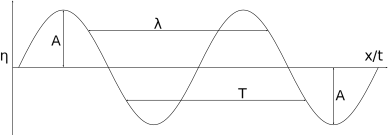
\includegraphics[width=\textwidth]{figures/sinusoid}
	\caption{Sample figure}
	\label{fig:sinusoid}
\end{figure}

It follows from equation~\ref{eq:sinusoid} that the surface elevation $\eta$ is limited by the amplitude $A$.
Moreover, for
\begin{equation}
kx - \omega t = const
\end{equation}
the surface elevation $\eta$ is always the same. We rewrite the term to
\begin{align}
x &= \frac{\omega}{k}t + \frac{const}{k} \\
t &= \frac{kx}{\omega}t - \frac{const}{\omega}
\end{align}
which gives us all positions $x$ or times $t$ the wave has the same value at.
%
\fxfatal{Add image}

\subsection{The Dispersion Relation}
\label{sec:dispersion_relation}

In linear wave theory there is a well known functional relationship between angular frequency~$\omega$
and wave number~$k$:
%
\begin{equation}
\label{eq:dispersion_relation}
 \omega^2 = gk\tanh(kd)
\end{equation}
%
where $g$ is the acceleration of earth's gravity and $d$ is the water depth. Equation~\ref{eq:dispersion_relation}
is called the~\emph{dispersion relation}.

There exist a useful set of modifications to the dispersion relation based on different conditions:
\begin{itemize}
 \item \emph{Shallow water approximation} - the water depth $d$ is much smaller than the wave length $\lambda$.
 \item \emph{Deep water approximation} - the water depth $d$ is much larger than the wave length $\lambda$.
\end{itemize}

In case of shallow water the respective dispersion relation is derived as follows:
\begin{align}
 d & \ll \lambda \\
 \Rightarrow 0 \leq kd & \ll 1 \\
 \Rightarrow \tanh(kd) & = kd \\
 \Rightarrow \omega^2 & = gk^2d
\end{align}

In contrast, for deep water the respective dispersion relation is reduced as follows:
\begin{align}
 d & \gg \lambda \\
 \Rightarrow kd & \gg 1 \\
 \Rightarrow \tanh(kd) & = 1 \\
 \Rightarrow \omega^2 & = gk
\end{align}

\subsection{Phase Velocity}
\label{sec:phase_velocity}
The rate at which a particular phase of a wave propagates in space is called the~\emph{phase velocity}.
The phase velocity is a vector and has an associated direction, the \emph{phase speed} on the other hand
refers only to the magnitude of the phase velocity. The most comprehensible example of phase speed
is rate of propagation of the wave crest. During one wave period $T$ the wave crest travels a distance
equal to the wave length $\lambda$. Let $c$ be the phase speed, then:
%
\begin{equation}
 c = \frac{\mathrm dx}{\mathrm dt} = \frac{\lambda}{T} = \frac{\omega}{k}
\end{equation}
%
As one can see, the phase speed is dependent on the dispersion relation. Given the dispersion relation
from equation~\ref{eq:dispersion_relation}, the phase speed is
\begin{equation}
 c = \sqrt{\frac{g}{k}\tanh{kd}}
\end{equation}

Given the dispersion relation
approximations for shallow and deep water in Section~\ref{sec:dispersion_relation}, the corresponding
phase speeds are derived as follows:
%
\begin{align}
 c &= \sqrt{gd} && \text{Shallow water phase speed}\\ \label{eq:phase_speed_shallow_water}
 c &= \sqrt{\frac{g}{k}} = \frac{g}{\omega} && \text{Deep water phase speed} \label{eq:phase_speed_deep_water}
\end{align}
%
In deep water the phase speed depends on the wave length (because of $k$) or the wave frequency (because of $\omega$).
Equation~\ref{eq:phase_speed_deep_water} implies that longer waves travel faster in deep water. Hence it is said, that
\emph{deep water waves are dispersive}. Shallow water waves, on the other hand, depend only on water depth, they are not considered
dispersive.

\subsection{Three Dimensional Wave}
Until now we were discussing a two dimensional ocean defined by exactly one sinus wave. As a first
step to get to a more realistic ocean surface representation we will extend equation~\ref{eq:sinusoid}
to form a wave in three dimensional space. In contrast to equation~\ref{eq:sinusoid}, where the wave's
travelling direction is fixed, the wave has to be able to travel in an arbitrary direction on a plane.
Moreover, we need to handle two dimensional input positions. The sinusoid describing surface elevation
in three dimensional space is defined as follows:
\begin{equation}
 \eta(\mvec{x}, t) = A\cos(\transpose{\mvec{k}}\mvec{x} - \omega t)
\end{equation}
where $\mvec{x} = (x_x, x_z)$ denotes the observed point on a plane and $\mvec{k} = (k_x, k_z)$ represents
the travelling direction of the wave. The wave number $k$ of wave vector $\mvec{k}$ is determined by the wave vector's
magnitude
\begin{equation}
 k = \norm{\mvec{k}}
\end{equation}
Thus, because of the dispersion relation, all waves of same magnitude share the same frequency.

\subsection{Sum of Waves}
Use euler identity for wave representation
\begin{equation}
 e^ix = \cos{x} + \mathrm{i}\sin{x}
\end{equation}
%
surface elevation looks as follows
%
\begin{equation}
 \eta(\mvec{x}, t) = \mathrm{Re}(A\mathrm{e}^{\mathrm{i}[\transpose{\mvec{k}}\mvec{x} - {\omega}t]})
\end{equation}
%
or equivalent
%
\begin{align}
 p &= A\mathrm{e}^{\mathrm{i}[\transpose{\mvec{k}}\mvec{x} - {\omega}t]} \\
 \eta &= \frac{1}{2}p + \frac{1}{2}p^*
\end{align}
where $p^*$ is the complex conjugate of $p$

Now the sum of waves
%
\begin{equation}
 \eta(\mvec{x}, t) = \sum_{\mvec{k}}a(\mvec{k})\mathrm{e}^{\mathrm{i}[\transpose{\mvec{k}}\mvec{x} - {\omega}t]}
\end{equation}
%
transform to
\begin{equation}
 \eta(\mvec{x}, t) = \sum_{\mvec{k}}B(\mvec{k})\mathrm{e}^{\mathrm{i}\transpose{\mvec{k}}\mvec{x}}
\end{equation}
%
we need $B(\mvec{k})$ for every $\mvec{x}$, which is not feasible
%
gaussian stationary process


\section{Statistical Wave Models}

\subsection{Phillips Spectrum}
\label{sec_phillips_spectrum}

\begin{align}
  k &= \norm{\mvec{k}}\\
  w &= \norm{\mvec{w}}\\
  P(\mvec{k}) &= A\frac{exp(-(kL)^{-2})}{k^4}\abs*{\frac{\transpose{\mvec{k}}}{k}\frac{\mvec{w}}{w}}^2\\
  P(\mvec{k}) &= A\frac{exp(-(kL)^{-2}-(kl)^2)}{k^4}\abs*{\frac{\transpose{\mvec{k}}}{k}\frac{\mvec{w}}{w}}^4
\end{align}


\subsection{Unified Spectrum}
\label{sec_unified_spectrum}

\section{The Projected Grid}
\label{sec_projected_grid}
The projected grid is based on a simple concept: in order to achieve an
uniform distribution of details on the image plane, a uniformly spaced grid is
created in post-perspective space and transformed back to world space.
Figure~\ref{fig:projectedgrid} illustrates the difference between a classic
world space approach and the projected grid.
\begin{figure}[h]
\centering
\subbottom[Classic]
{
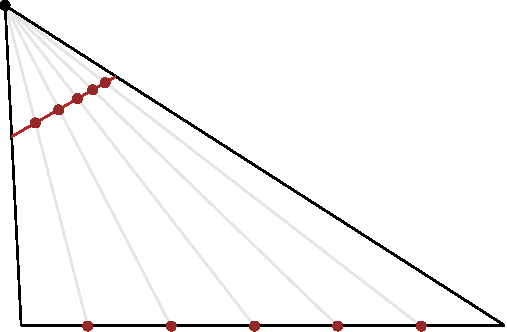
\includegraphics[scale=0.75]{figures/ProjectedGridVsWorldSpace.pdf}
\label{fig:subfigprojgrid1}
}
\subbottom[Projected Grid]
{
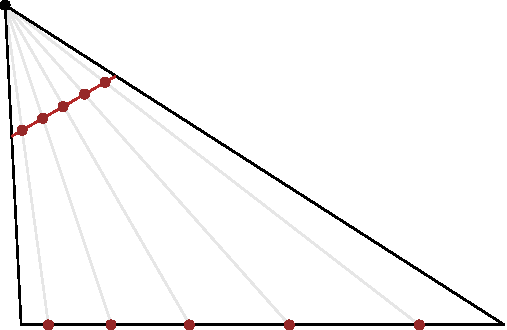
\includegraphics[scale=0.75]{figures/ProjectedGridUniform.pdf}
\label{fig:subfigprojgrid2}
}
\caption{The image on the left shows an uniform grid in worldspace,
its projection onto the image plane is not uniformly spaced though.
The image on the right on the other hand depicts an uniform grid on
the image plane and its associated non-uniform spaced worldspace
positions.}
\label{fig:projectedgrid}
\end{figure}

% The algorithm used for the projected grid can be broken down into the following
% steps:
% \begin{itemize}
%  \item create a uniformly spaced grid orthogonal to the viewer using normalised
% device coordinates
%  \item transform the grid to worldspace
%  \item project the grid onto the desired base plane
%  \item apply height displacement
%  \item run the grid through the rendering pipeline as usual
% \end{itemize}

\subsection{Coordinate Systems}
\label{sec:coordinate_systems}
Let $\mvec{x}$ be a vector representing the three dimensional carthesian
world space coordinate of a vertex, then
\begin{equation}
 \mvec{w} = \transpose{(\mvecx{x}, \mvecy{x}, \mvecz{x}, 1)}
\end{equation}
where $\mvec{w}$ is a homogeneous world space coordinate of $\mvec{x}$.
Let $\mmat{V}$ be the view matrix and $\mmat{P}$ the projection matrix, then
\begin{equation}
\label{eq:ws_to_cs}
 \mvec{c} = \mmat{P} \mmat{V} \mvec{w}
\end{equation}
where $\mvec{c}$ is the \textit{clip space} coordinate of $\mvec{w}$. For $\mvec{c}$ to
be inside the view frustum defined by $\mmat{P}$, $\mvec{c}$ is required to
meet the following condition
\begin{equation}
\label{eq:cs_bounds}
 \mvecx{c}, \mvecy{c}, \mvecz{c} \in \interval{-\mvecw{c}}{\mvecw{c}}
\end{equation}
where $\mvecw{c}$ is the homogeneous component of $\mvec{c}$. Next, clip space
vertex $\mvec{c}$ is transformed by the \textit{perspective division} as follows
\begin{equation}
\label{eq:cs_to_ndc}
 \mvec{n} = \frac{1}{\mvecw{c}}\transpose{(\mvecx{c}, \mvecy{c}, \mvecz{c})}
\end{equation}
where $\mvec{n}$ corresponds to the \textit{normalised device coordinate},
\textit{NDC} in short, of $\mvec{c}$.
%
%
\begin{figure}
\centering
\subbottom[View Frustum]
{
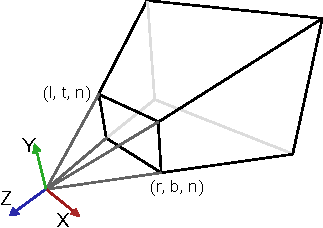
\includegraphics[width=0.4\textwidth]{figures/ProjectiveFrustum.pdf}
\label{fig:subfig_proj_frustum}
}
\subbottom[Canonical view volume]
{
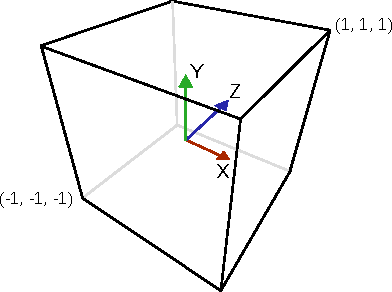
\includegraphics[width=0.4\textwidth]{figures/CanonicalCube.pdf}
\label{fig:subfig_canonical_view_volume}
}
\caption{Left: An example view frustum in view space. Right: The same view frustum
after applying projection and perspective division.}
\label{fig:proj_frustum_ndc}
\end{figure}
%
%
As one can see, equations~\ref{eq:cs_bounds}
and~\ref{eq:cs_to_ndc} imply
\begin{equation}
\label{eq:ndc_bounds}
 \mvecx{n}, \mvecy{n}, \mvecz{n} \in \interval{-1}{1}
\end{equation}
which defines the space NDC reside in, namely the \textit{canonical view volume},
see Figure~\ref{fig:proj_frustum_ndc}.\\


The projected grid, on the other hand, starts inside the canonical view volume
and needs to transform vertices back to world space. Let $\mvec{n}$ be the
normalised device coordinate of a vertex, then
\begin{equation}
\label{eq:ndc_to_cs}
 \mvec{c} = \transpose{(\mvecx{n}, \mvecy{n}, \mvecz{n}, 1)}
\end{equation}
where $\mvec{c}$ is a valid representation of $\mvec{n}$ in clip space. One may choose
a value for $\mvecw{c}$ different from $1$, making it necessary to scale $\mvecx{n}$,
$\mvecy{n}$ and $\mvecz{n}$ accordingly. Again, let $\mmat{V}$ be the view matrix and
$\mmat{P}$ the projection matrix, then
\begin{equation}
\label{eq:cs_to_wsh}
 \mvec{w} = \inverse{(\mmat{P} \mmat{V})} \mvec{c}
\end{equation}
where $\mvec{w}$ is a homogeneous world space coordinate of $\mvec{c}$. Conversion
to three dimensional carthesian world space is accomplished as follows
\begin{equation}
\label{eq:wsh_to_ws}
 \mvec{x} = \frac{1}{\mvecw{w}}\transpose{(\mvecx{w}, \mvecy{w}, \mvecz{w})}
\end{equation}

\subsection{Projection onto Plane}
As noted before, the vertices of the projected grid are represented as normalised
device coordinates. Assuming the plane the grid shall be projected on is specified
in world space coordinates, the following steps need to be computed for each vertex:
\begin{itemize}
 \item Transform vertex from canonical view volume to world space
 \item Setup vertex specific ray
 \item Intersect ray with target plane to compute actual position
\end{itemize}
Step one is already covered by Section~\ref{sec:coordinate_systems}. Step two
requires to setup a ray for each vertex, which implies both a position and a
direction. The position we already have, but to create a direction we need two
different positions. The solution is rather straightforward: let $\mvec{n}$ be
a \textit{two dimensional} vector representing the \textit{X} and \textit{Y}
components of a position in normalised device coordinates, then
\begin{align}
 \mvec{a} & = (\mvecx{n}, \mvecy{n}, -1, 1)\\
 \mvec{b} & = (\mvecx{n}, \mvecy{n}, +1, 1)
\end{align}
where $\mvec{a}$ corresponds to $\mvec{n}$ on the \textit{near plane} in clip space,
and $\mvec{b}$ to $\mvec{n}$ on the \textit{far plane} in clip space. Let $\mvec{d}$
and $\mvec{e}$ be the carthesian world space positions of $\mvec{a}$ and $\mvec{b}$
respectively, then
\begin{equation}
 \label{eq:proj_grid_ray}
 \mvec{p} = \mvec{d} + t(\mvec{e} - \mvec{d})
\end{equation}
where $\mvec{p}$ represents a ray starting at point $\mvec{d}$, pointing in direction
$(\mvec{e} - \mvec{d})$ with variable parameter $t$ controlling the actual position on
the ray.\\

Step three is about intersecting ray $\mvec{p}$ resulting from step two with the target plane.
We define the target plane using the \textit{Hesse normal form} as follows
\begin{equation}
\label{eq:proj_grid_plane}
 \mvec{p}\transpose{\mvec{n}} - d = 0
\end{equation}
where $\mvec{n}$ is the plane's normal vector with unit length and $d$ the plane's distance
from the origin. Next, we insert $\mvec{p}$ from equation~\ref{eq:proj_grid_ray}
into equation~\ref{eq:proj_grid_plane}, resulting in
%
\begin{gather}
\label{eq:plane_and_ray_intersection}
(\mvec{d} + t(\mvec{e} - \mvec{d})\transpose{\mvec{n}} - d = 0\\
\mvec{d}\transpose{\mvec{n}} + t(\mvec{e} - \mvec{d})\transpose{\mvec{n}} - d = 0\\
\intertext{solve for $t$}
t = \cfrac{d - \mvec{d}\transpose{\mvec{n}}}{(\mvec{e} - \mvec{d})\transpose{\mvec{n}}}
\end{gather}
%
where $t$ in combination with equation~\ref{eq:proj_grid_ray} gives the point of intersection
between the ray and the plane. In case $(\mvec{e} - \mvec{d})\transpose{\mvec{n}} = 0$,
there is no point of intersection because the ray is parallel to the plane.

\subsection{Projector}
\fxnote*{JÖSSAS}{Backfiring, etc}